\documentclass{article}

% if you need to pass options to natbib, use, e.g.:
% \PassOptionsToPackage{numbers, compress}{natbib}
% before loading nips_2016
%
% to avoid loading the natbib package, add option nonatbib:
% \usepackage[nonatbib]{nips_2016}

% \usepackage{nips_2016}

% to compile a camera-ready version, add the [final] option, e.g.:
\usepackage[final]{nips_2016}

\usepackage[utf8]{inputenc} % allow utf-8 input
\usepackage[T1]{fontenc}    % use 8-bit T1 fonts
\usepackage{hyperref}       % hyperlinks
\usepackage{url}            % simple URL typesetting
\usepackage{booktabs}       % professional-quality tables
\usepackage{amsfonts}       % blackboard math symbols
\usepackage{nicefrac}       % compact symbols for 1/2, etc.
\usepackage{microtype}      % microtypography
\usepackage{listings}
\usepackage{graphicx}

\graphicspath{ {figures/} }

\title{Applying Temporal Difference Learning Methods to Machine Learning}

% The \author macro works with any number of authors. There are two
% commands used to separate the names and addresses of multiple
% authors: \And and \AND.
%
% Using \And between authors leaves it to LaTeX to determine where to
% break the lines. Using \AND forces a line break at that point. So,
% if LaTeX puts 3 of 4 authors names on the first line, and the last
% on the second line, try using \AND instead of \And before the third
% author name.

\author{
  Philippe Lacaille \\
  Reinforcement Learning Final Project \\
  COMP 767 - McGill - Winter 2017 \\
  \texttt{philippe.lacaille@umontreal.ca} \\
  %% examples of more authors
  %% \And
  %% Coauthor \\
  %% Affiliation \\
  %% Address \\
  %% \texttt{email} \\
  %% \AND
  %% Coauthor \\
  %% Affiliation \\
  %% Address \\
  %% \texttt{email} \\
  %% \And
  %% Coauthor \\
  %% Affiliation \\
  %% Address \\
  %% \texttt{email} \\
  %% \And
  %% Coauthor \\
  %% Affiliation \\
  %% Address \\
  %% \texttt{email} \\
}

\begin{document}
% \nipsfinalcopy is no longer used

\maketitle

\begin{abstract}
  Temporal Difference learning methods were introduced in 1988 and they have been the foundation of Reinforcement Learning algorithms ever since. When introduced, these methods were not specially intended at RL problems but rather generally proposed as a learning framework for any prediction problems. This paper serves as a report for my case study on applying such TD methods to multi-steps prediction problems usually handled by supervised Machine Learning. This report is a mirror of the series of posts I published on my blog while working on this project (\url{https://placailleblog.wordpress.com/category/courses/reinforcement-learning-mcgill-comp767/project-td-methods-for-ml/}).

  All code used to generate results can be found at the following GitHub repo\\ \url{https://github.com/rllabmcgill/rlcourse-final-project-placaille}.
\end{abstract}

\section{Introduction}

When introducing these methods, Sutton \cite{sutton1988learning} makes the claim that temporal-difference methods have an advantage over typical supervised learning because it has the effect of spreading out the computation load and generate more accurate predictions.

He emphasizes that this is true in a particular setting where the predictions are for multi-step prediction problems, meaning what we are trying to predict is only revealed after a sequence of predictions. In a sense, problems where we can only know the true outcome after multiple steps have been observed and predicted.

The author even further argues these types of problems occur more often in the real-world rather than single-step prediction problems, where each time a prediction is made, the real outcome can be verified.

Here are some examples of multi-steps prediction problems

\begin{itemize}
  \item Monthly predictions for the end-of-year financial results of a company
  \item Daily predictions for rain on the upcoming Saturday
  \item Class prediction at each second for a video clip
\end{itemize}

What I propose in this case study is to play with a classic machine learning problem that is the MNIST dataset. I will detail further along how this problem can be modified to be considered a multi-step prediction problem. In addition, in the following sections I will be showing the theoretical background and empirical results that support this approach. I will also show results of the intra-sequence updating rule variant of TD learning with the same task.

\section{Temporal Difference Learning}

The main concept behind the temporal-difference learning methods is to allow feedback to be learned based on the differences of the predictions that are made at each step, as opposed to waiting for the real outcome at the end of a sequence of observations.

Let's consider a sequence of observations $x_1, x_2, \dots, x_m$ that lead to the outcome $z$. Let's further denote the prediction of $z$ at each time step $t \in \{1, \dots, m\}$ as $P_t$, and where $P_{m+1} = z$. In addition, $x_t$ could denote an observation vector of different attributes. We are therefore trying to predict what will be the final outcome after each observation $x_t$ at time $t$. To do so, we will be using a set of weights denoted $w$, where $P_t$ can now be written as $P(x_t, w)$. Sutton analyses the case where $P(x_t, w)$ is a linear function of $x_t$ and $w$. I will be exploring the non-linear case further down the line when being applied to MNIST.

For now, let's focus on a variant of this problem where the weights are only updated at the end of the sequence under the following update rule,

$w \leftarrow w + \sum \limits_{t=1}^m \Delta w_t$

\subsection{Traditional supervised learning approach}

Under the traditional supervised learning approach, all observations $\{ x_1, x_2, \dots, x_m \}$ are considered paired observations with the outcome $z$. Under this approach, and given our prediction function $P(x_t, w)$ a very popular gradient update rule for $w$ based on backpropagation of the error can be given by the following,

$\Delta w_t = \alpha (z - P_t) \nabla_w P_t$

Where $\nabla_w P_t$ is the gradient of the prediction at time $t$ with regard to the weights of our function and $\alpha$ our learning rate.

An important observation that the author emphasizes is the fact that all $\Delta w_t$ for all $t$ depend on the error at each time step $(z - P_t)$ which themselves depend on $z$ that is only known at the end of the sequence under the types of problems that we are exploring. In practical terms, we would therefore make a prediction and determine the gradient at each time step, store them in memory until the end of the full sequence and once the outcome is known, compute the errors at each time step and do the update to our weights.

This is what TD learning will aim to circumvent, to allow iterative calculations to be made rather than stacking up the information in other to reduce the memory requirements.

\subsection{TD approach}
The main issue with the traditional machine learning approach described above is the update rule referring to the real outcome at each time step. Sutton suggests that rather to see the error as the outcome vs our current predictions, to consider the sum of all differences between our future predictions that will occur $(P_{t+1} - P_t)$. These differences in predictions at each time steps are called temporal differences, hence the name of the method!

Now let's do a bit of math to figure out what would be the update rule based on this approach.

Arithmetically, we can rewrite $z - P_t$ as $\sum \limits_{k=t}^m(P_{k+1} - P_k)$, where $P_{m+1} = z$. We can then re-write the update rule from the first approach,

$w \leftarrow w + \sum \limits_{t=1}^m \alpha (z - P_t) \nabla_w P_t = w + \sum \limits_{t=1}^m \alpha \sum \limits_{k=t}^m (P_{k+1} - P_k) \nabla_w P_t$

By following Fubini's theorem, we can switch the indices of the double summation to obtain

$w + \sum \limits_{t=1}^m \alpha \sum \limits_{k=t}^m (P_{k+1} - P_k) \nabla_w P_t = w + \sum \limits_{k=1}^m \alpha \sum \limits_{t=1}^k (P_{k+1} - P_k) \nabla_w P_t$.

By simply swapping the indices $k$ and $t$ for clearer understanding and moving around constants, we can finally obtain the update rule,

$w \leftarrow w + \sum \limits_{t=1}^m \alpha (P_{t+1} - P_t) \sum \limits_{k=1}^t \nabla_w P_k$

We can then see this update rule as a sum of $\Delta w_t$ for any $t$ as,

$\Delta w_t = \alpha (P_{t+1} - P_t) \sum \limits_{k=1}^t \nabla_w P_k$.

We can therefore notice the update rule for the TD approach doesn't require the actual outcome $z$ (unless on the last prediction $m$). It therefore doesn't require us to track all the predictions that were made during the sequence. To compensate though, we need to compute the sum of gradients over previous time steps, which can be done easily in terms of memory, as we can only store the current sum and add the current gradient when obtained.

In other words, when we compute the predictions at time step $t+1$, we can obtain the sum of previous updates easily. We determine the TD error $(P_{t+1} - P_t)$, simply add the gradient to the total gradient kept in memory w.r.t. the weights and increment our sum of updates. When we reach the end of the sequence, no additional computation than any previous step is required other than doing the actual updates to $w$.

This dramatically reduces the memory requirements compared to the traditional machine learning approach detailed above, especially in cases of long sequence.

\section{Using MNIST as a multi-step prediction problem}

Traditionally MNIST has been seen as a single-step prediction problem, i.e. we see the 28x28 pixel input as a whole, compute a prediction and compare it to the real number. In order to use it as a multi-step prediction problem, we can simply consider the image input as a sequence of 784 pixels! This way, after each pixel if observed, we can make a prediction w.r.t. the image and have the real outcome once the image has been fully covered, making it a multi-step prediction problem.

Indeed, we can therefore denote pixel $i$ as $p_i$ and going from left to right and from top row to bottom row, we can obtain a sequence $p_1, p_2, \dots, p_{784}$. We can further denote the outcome of the sequence as being the class of the image $z \in \{ 0, 1, 2, \dots, 9 \}$.

Additionally, to make the computation of the prediction $P_t$ at time step $t$ a function of all previously observed pixels in the sequence rather than just the current pixel $p_t$, we can express our observation at time $t$ as $x_t = [p_1, p_2, \dots, p_{t-1}, p_t, 0, \dots, 0, 0]^T$ as being a vector of size 784 with all previously seen pixels up to time step $t$ and 0 afterwards.

An important consideration with regard to the problem I am using to apply TD learning methods is TD learning uses the mean squared error (MSE) as its loss function. The MNIST dataset is usually used as a classification task and implicitly the cross-entropy as its loss function. Even though using the MSE isn't optimal, it can still be applied by considering MNIST as a regression problem on the class number.

%%%%%%%%%%

\section{Traditional approach}

After considering the sequence problem, the ML traditional implementation is similar to the Monte Carlo approach. In a sense, at each step we make a prediction for the outcome, store it, and once at the end of the sequence, we go through all our predictions, compare it to the true outcome and make an update to our parameters.

In order to simplify and increase the speed, rather than considering each pixel as a time step, I consider each row of pixels as a time step. Since each input is originally 28x28 pixels, we therefore have sequences of 28 time steps.

\pagebreak

Here is an excerpt of my code showing the procedure

\begin{lstlisting}[language=Python]
  for t in xrange(784):

      # apply mask at fixed interval, making sequences of pixels appear
      if (t + 1) % 28 == 0:
          nb_seq += 1

          seq_x = train_x * mask[t]
          pred_y = predict(seq_x)
          grad = preds_grad(seq_x)

  # update params based on experience
  old_param_values = lyr.get_all_param_values(network)
  new_param_values = old_param_values

  for pred, grad in zip(batch_preds, batch_grads):

      error = (true_y - pred)
      delta_params = LRN_RATE * error * grad
      new_param_values += delta_params
      batch_error.append(error)

  lyr.set_all_param_values(network, new_param_values)
\end{lstlisting}

To consider this as a multi-step prediction problem, we need to assume the real outcome is only available at the end of the sequence. This is why the true outcome is only used after the sequence has been explored. The important component is the following, which is calculated for each $t$ in our sequence.

\begin{lstlisting}[language=Python]
  error = (true_y - pred)
  delta_params = LRN_RATE * error * grad
\end{lstlisting}

We can notice we always refer to the true outcome for updating our parameters, which makes it without any bias, but still doesn't bootstrap the updates with its own predictions.

\subsection{Results}

To relate this problem with reinforcement learning, we can consider an example from the dataset as being an episode that the agent experiences.

Below is the plot of the running average of the L2 norm of the error sequence over 4 iterations of the dataset. The error sequence refers to the error that is made at each time step during a sequence (the lower the better).

\begin{center}
  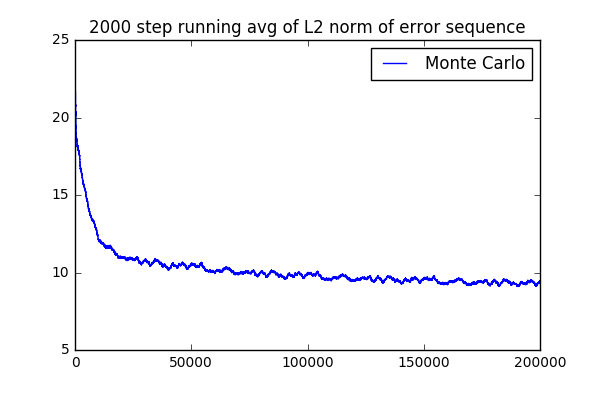
\includegraphics[width=75mm]{figures/plot_MC_L2_norm_error.png}
\end{center}

These results labeled as Monte Carlo will be the baseline results under the traditional approach for further comparison.

\section{Temporal Difference approach}

Now let's consider the approach discussed where we can determine the updates by only considering the TD errors (errors between subsequent predictions) to determine the update to our parameters. For this approach, we will need to modify our previous code in order to track the sum of gradients up to the current time step, and also determine the error based on the following prediction.

As a reminder, here is the equation for our parameter update coming from time step $t$.

$\Delta w_t = \alpha (P_{t+1} - P_t) \sum \limits_{k=1}^t \nabla_w P_k$.

Here is the same part of my code but under the TD approach.

\begin{lstlisting}[language=Python]
  old_param_values = lyr.get_all_param_values(network)
  new_param_values = old_param_values

  for t in xrange(784):

    # apply mask at fixed interval, making sequences of pixels appear
    if (t + 1) % 28 == 0:

        nb_seq += 1

        seq_x = train_x * mask[t]
        pred = predict(seq_x)[0, 0]
        grad = preds_grad(seq_x)

        if nb_seq == 1:
            sum_grad = np.copy(grad)
        else:
            sum_grad += np.copy(grad)

        if t < 783:
            seq_x_prime = train_x * mask[t + 28]
            pred_y_prime = predict(seq_x_prime)[0, 0]
            TD_error = (pred_y_prime - pred)
            error = (true_y - pred)
        else:
            TD_error = (true_y - pred)
            error = (true_y - pred)

        delta_params = LRN_RATE * TD_error * sum_grad
        new_param_values += delta_params
        batch_error.append(error)

  # update params based on experience
  lyr.set_all_param_values(network, new_param_values)
\end{lstlisting}

You might notice I am still tracking the true error, and it is for comparison purposes to the other method. Otherwise, the TD error cannot be compared to the true error.

We can notice now that rather than having a delta parameter at time step $t$ based on the current error and current gradient, we have the following,

\begin{lstlisting}[language=Python]
  TD_error = (pred_y_prime - pred)
  [...]
  delta_params = LRN_RATE * TD_error * sum_grad
\end{lstlisting}

Due to the change in procedure, there is a gain in memory since we no longer have to keep the predictions in memory during an episode/sample.

\subsection{Results}

As previously described, we should expect this method to generate the same results as for the previous approach. This is true because our modified update rule was obtained from the same source and no bias was introduced.

In order to compare both methods, I show the running average of the L2 norm of the error sequence just like the previous approach. In addition, both methods superposed are showed in the right figure (this time average is over the full length of the training).

\begin{center}
  \begin{minipage}{.5\textwidth}
    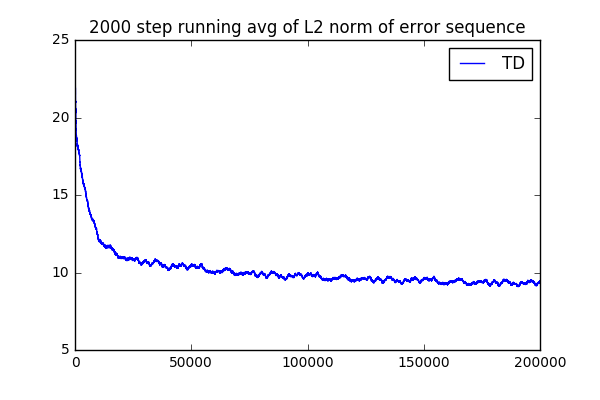
\includegraphics[width=\linewidth]{figures/plot_TD_L2_norm_error.png}
  \end{minipage}%
  \begin{minipage}{.5\textwidth}
    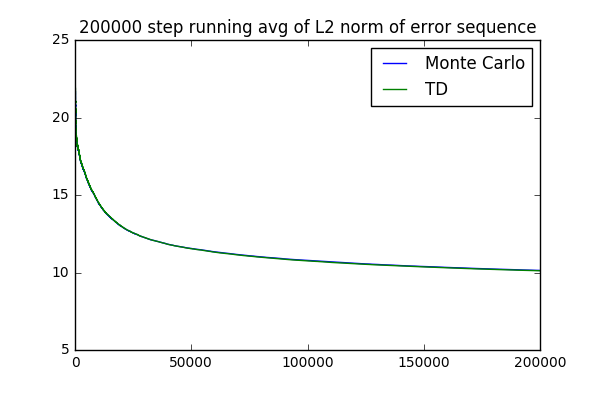
\includegraphics[width=\linewidth]{figures/plot_both_L2_norm_error.png}
  \end{minipage}
\end{center}

We can therefore see the Temporal Different approach proposed by Sutton indeed produces the same results while having a memory advantage of not having to store ongoing predictions.

This is because both of these do generate the same parameter updates, but also both of these methods only update the parameters after the sequence is over.

\section{Intra-sequence parameter updating}

The true essence of the TD learning methods evolves around intra-sequence parameters updating. Sutton sums it best in the original TD learning paper.

\begin{quote}
  Since each observation of a sequence generates an increment to the weight vector, in many respects it would be simpler to update the weight vector immediately after each observation.
\end{quote}

Indeed, could we find a way not to wait at the end of a sequence to update the parameters? This could potentially help us converge more quickly and require less episodes/examples. Sutton mentions the most intuitive update rule would be the following update rule at each time step $t$,

$w_{t+1} = w_t + \alpha(P_{t+1} - P_t) \sum \limits_{k=1}^t \nabla_w P_k$ where $P_t = P(x_t, w_{t-1})$

Similarly to the method where we update only at the end of the sequence, the change of parameters would be function of the current TD error and the cumulative sum of gradients. In addition, each prediction would be function of the previous set of parameters.

But as the author points out, this has the problem where the observed TD error $P_{t+1} - P_t$, is a function of a change in parameters as well as the new observation at $t+1$. Ideally, we would like to have only the impact of the new observation in the TD error.

\section{Fixing the parameters}

One recommendation Sutton proposes to alleviate the dependance of the TD error to the parameter change, is to make the prediction at time step $t+1$ with the current set of parameters before updating it. The full proposed update rule is the following,

$w_{t+1} = w_t + \alpha(P(x_{t+1}, w_t) - P(x_t, w_t)) \sum \limits_{k=1}^t \nabla_w P(x_k, w_t)$

Under this approach, we would therefore determine the TD error according to our current set of parameters. On the next time step, the predictions for the TD error are redetermined based on the newly updated parameters.

\begin{lstlisting}[language=Python]
  for t in xrange(784):

    # apply mask at fixed interval, making sequences of pixels appear
    if (t + 1) % 28 == 0:

        nb_seq += 1

        seq_x = train_x * mask[t]
        pred = predict(seq_x)[0, 0]
        grad = preds_grad(seq_x)

        if nb_seq == 1:
            sum_grad = np.copy(grad)
        else:
            sum_grad += np.copy(grad)

        if t < 783:
            seq_x_prime = train_x * mask[t + 28]
            pred_y_prime = predict(seq_x_prime)[0, 0]
            TD_error = (pred_y_prime - pred)
            error = (true_y - pred)
        else:
            TD_error = (true_y - pred)
            error = (true_y - pred)

        param_values = lyr.get_all_param_values(network)
        delta_params = LRN_RATE * TD_error * sum_grad
        param_values += delta_params
        lyr.set_all_param_values(network, param_values)
\end{lstlisting}

One important component to notice is the fact that the sum of the gradients up to time step $t$ is still needed to evaluate the update. This makes it more computationally intensive than the original TD learning method previsouly explored since we are computing the same things, but actually doing the update during the sequence.

\subsection{Results}

Another thing to point out is that all the methods so far have been using the full sequence of gradients, which are analogous to Monte Carlo method. For clarity, this method has been labeled as \textit{TD incr.}.

The following graph shows the same metric as before but for the incremental TD rule (including previous methods).

\begin{center}
  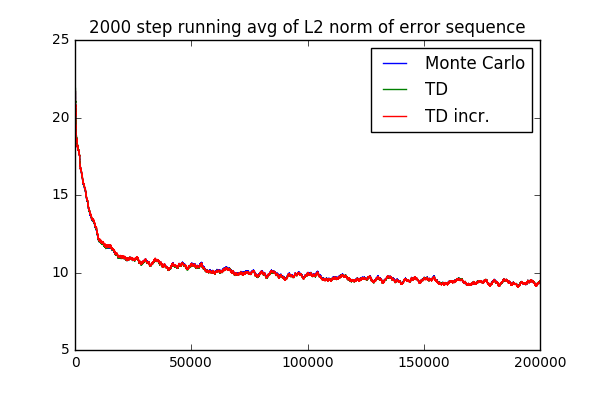
\includegraphics[width=75mm]{figures/plot_TD_incr_grad_L2_norm_error.png}
\end{center}

We can notice the performance is once again the same as the previous methods. This is the case because we have the full lengths of the gradient of the sequence to make the update. This is an interesting results as we are using the one-step prediction as the error feedback, but by considering all previous gradients with intra-sequence updates we are having the same updates.

However for the task explored, we are basically requiring more computations at each time step, while still obtaining the same performance as waiting at the end of the sequence. There is therefore not much benefits to use this new method.

In the following section, we will see how not using the full sequence of gradients affects the performance.

\section{One-step updates}

The next improvement that can be thought of is to actually not require all the previous history of gradients and rather only focus on the last one. This methods can be seen analogous to TD(0). The update rule now becomes the following,

$w_{t+1} = w_t + \alpha(P(x_{t+1}, w_t) - P(x_t, w_t)) \nabla_w P(x_t, w_t)$

Here is an excerpt from my code with this approach implemented,

\begin{lstlisting}[language=Python]
  for t in xrange(784):

      # apply mask at fixed interval, making sequences of pixels appear
      if (t + 1) % 28 == 0:

          nb_seq += 1

          seq_x = train_x * mask[t]
          pred = predict(seq_x)[0, 0]
          grad = preds_grad(seq_x)

          if t < 783:
              seq_x_prime = train_x * mask[t + 28]
              pred_y_prime = predict(seq_x_prime)[0, 0]
              TD_error = (pred_y_prime - pred)
              error = (true_y - pred)
          else:
              TD_error = (true_y - pred)
              error = (true_y - pred)

          param_values = lyr.get_all_param_values(network)
          delta_params = LRN_RATE * TD_error * grad
          param_values += delta_params
          lyr.set_all_param_values(network, param_values)
\end{lstlisting}

This now becomes a compromise of increased efficiency while introducing a bias in our update. In practice, this method is not guaranteed to converge when using non-linear approximation such as a small neural network in this case study.

\subsection{Results}

Below are is the results for one-step updates where only the recent gradient is considered. The other method's results have been included for comparison.

\begin{center}
  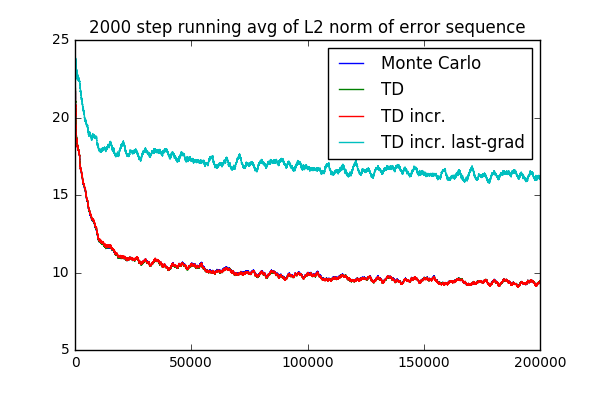
\includegraphics[width=75mm]{figures/plot_TD_last_grad_L2_norm_error.png}
\end{center}

The thing that can be clearly seen is how this approach underperforms compared to the full updates previously seen. This is quite disappointing because it is the most memory efficient compared to other methods.

It can be explained simply that when we used the full sum of gradients update, we have much more information to provide to our weight updates. Therefore it will be faster to converge. Under the one-step update, we only have the current gradient to propagate. It seems that the single-step updates does not help the performance on this task.

\section{Thoughts}

The main takeaway from this case study is that the first TD method explored (the one with an update at the end of the sequence) only offers greater benefits than the traditional machine learning approach at no additional cost. This slight modification to the update rule allows to save on memory while still making the same updates.

The question also can be raised with regard to applying intra-sequence updates for a more complexe model such as the family of Recurrent Neural Networks (RNNs). However, the loss implied by the type of tasks usually associated to RNNs isn't the MSE and couldn't benefit from the modification initially proposed by Sutton.

Some possible direction to expand on is to consider the full TD($\lambda$) family of algorithms where the sum of gradients is a geometrically weighted sum of previous gradients. Eligibility traces which are an extension of the TD($\lambda$) family of algorithms could potentially help. This has proven under traditional reinforcement learning tasks to increase performance.

\bibliography{project_ref}
\bibliographystyle{plain}

\end{document}
